\section{Graphical User Interface}
The Graphical User Interface (GUI) is designed in such a way that it can
accommodate the various usage scenarios common for this tool.  Therefore, it
must bridge the gap between simplicity and complexity so that users can simply
use the tool and power users can use the tool to create powerful system-altering
scripts.

The GUI is inspired by the well-known Windows application installer paradigm. 
Basic users will only encounter screens similar to what they are familiar with
when installing or uninstalling applications.  The interface will become much
more complex when power users use the tool to modify scripts, but this is to be
expected.  The editing script interface is inspired by tools that exist in the
field (namely OTA and HijackThis).

\subsection{Main}
When a user opens the application, they must be presented with the screen from
Figure~\ref{fig:gui_main}.  This screen is the decision point of the
application.  Depending on the user's input, this screen will take the user
through the workflows of this tool.

\begin{figure}[h]
  	\centering
	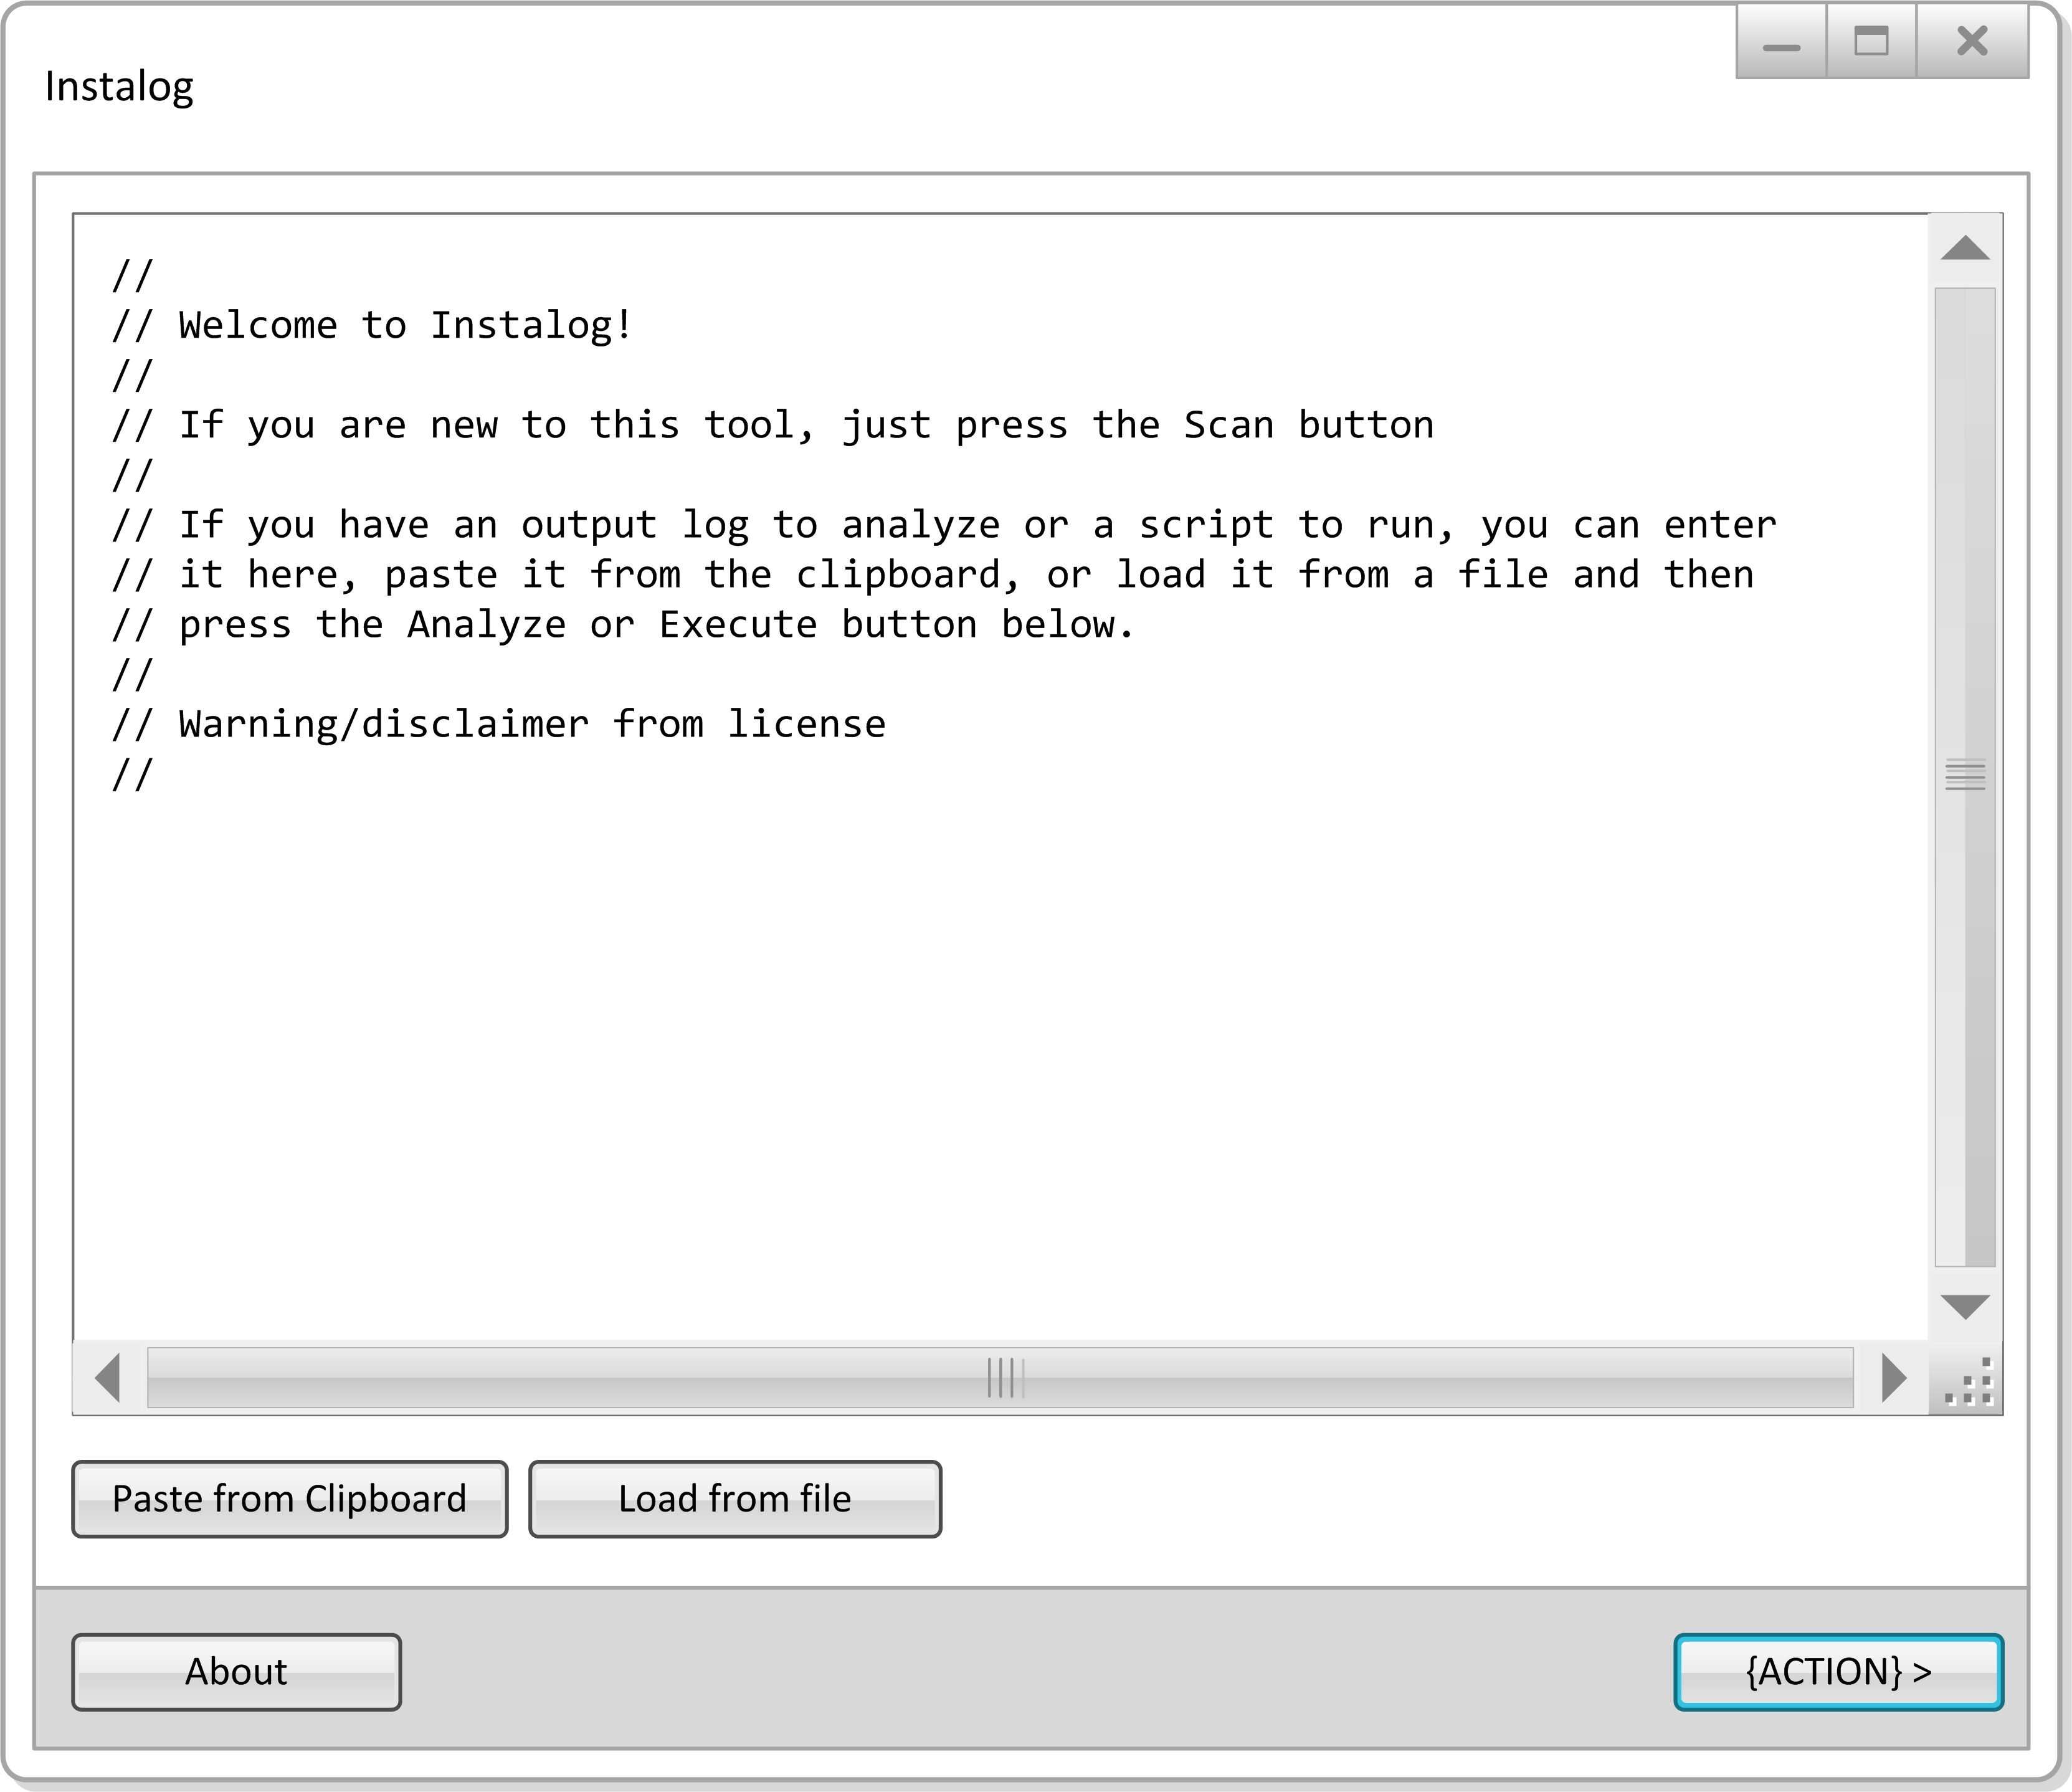
\includegraphics{figures/gui/Main.png}
  	\caption{GUI Main Screen}
  	\label{fig:gui_main}
\end{figure}

\begin{description}
\item[Textbox requirements] \hfill
\begin{enumerate}
\item The textbox shall support basic operations including but not limited to
Copy, Paste, and Undo/Redo.
\item Thee textbox shall not implement word-wrap.	  
\end{enumerate}

\item[Paste from Clipboard button requirements] \hfill
\begin{enumerate}
\item This button shall clear the contents of the textbox and then place
the full contents of the clipboard into the textbox
\item If the clipboard does not contain text data, this button must be
disabled
\end{enumerate}

\item[Load from File button requirements] \hfill
\begin{enumerate}
\item Pressing this button will the standard Windows file open dialog.  It
shall be enabled for searching for \texttt{*.txt} and \texttt{*.zip} files.
\begin{enumerate}
\item  If a valid file is opened, the contents of the textbox shall be cleared
and then the full contents of the file shall be placed into the textbox.
Obviously, zipped files should be unzipped.
\item If the user presses cancel in the dialog, the contents of the textbox
shall not be changed
\end{enumerate}
\end{enumerate}

\item[\var{action} button requirements] \hfill
\begin{enumerate}
\item The contents of the textbox shall be scanned to determine if it contains
default script content (or empty script content), script content, or log
content.  If so, the button shall display ``Scan," ``Execute," or ``Analyze"
(respectively).
\item The button shall have differing behavior based on the inferred content of
the textbox:
\begin{enumerate}
\item If the button reads ``Scan," the tool shall proceed to the Running Screen
(section~\ref{sec:running_screen}) running the default script
(section~\ref{sec:default_script_sections}).
\item If the button reads ``Execute," the tool shall proceed to the Running
Screen (section~\ref{sec:running_screen}) running the supplied script.
\item If the button reads ``Analyze," the tool shall proceed to the Analysis
Screen (section~\ref{sec:analysis_screen}) displaying the parsed log.
\end{enumerate}
\item If the type of the content in the textbox cannot be inferred or the
content of the textbox is not syntactically valid, the button shall display
the text of the last inferred \var{ACTION}.  If the user presses the
\var{ACTION} button for an invalid script, the applicaiton must not continue. 
Instead, an error message must appear that informs the user that the script is
invalid and therefore the tool will not continue.
\end{enumerate}

\item[About button requirements] \hfill
\begin{enumerate}
\item This button shall display a screen that contains the license for this
project (section~\ref{sec:licensing}) as well as information for any other
tools used in this project.  This screen shall have a simple close button.
\item The behavior for this button is the same on all following windows. 
\end{enumerate}
\end{description}

\subsection{Running Screen} \label{sec:running_screen}
This screen will run a script.  For the purpose of these requirements, it is not
important whether the script is the default script or a custom script.  The
script shall automatically begin when this screen is displayed.  The Running 
Screen is presented in Figure~\ref{fig:gui_running}.

\begin{figure}[h]
  	\centering
	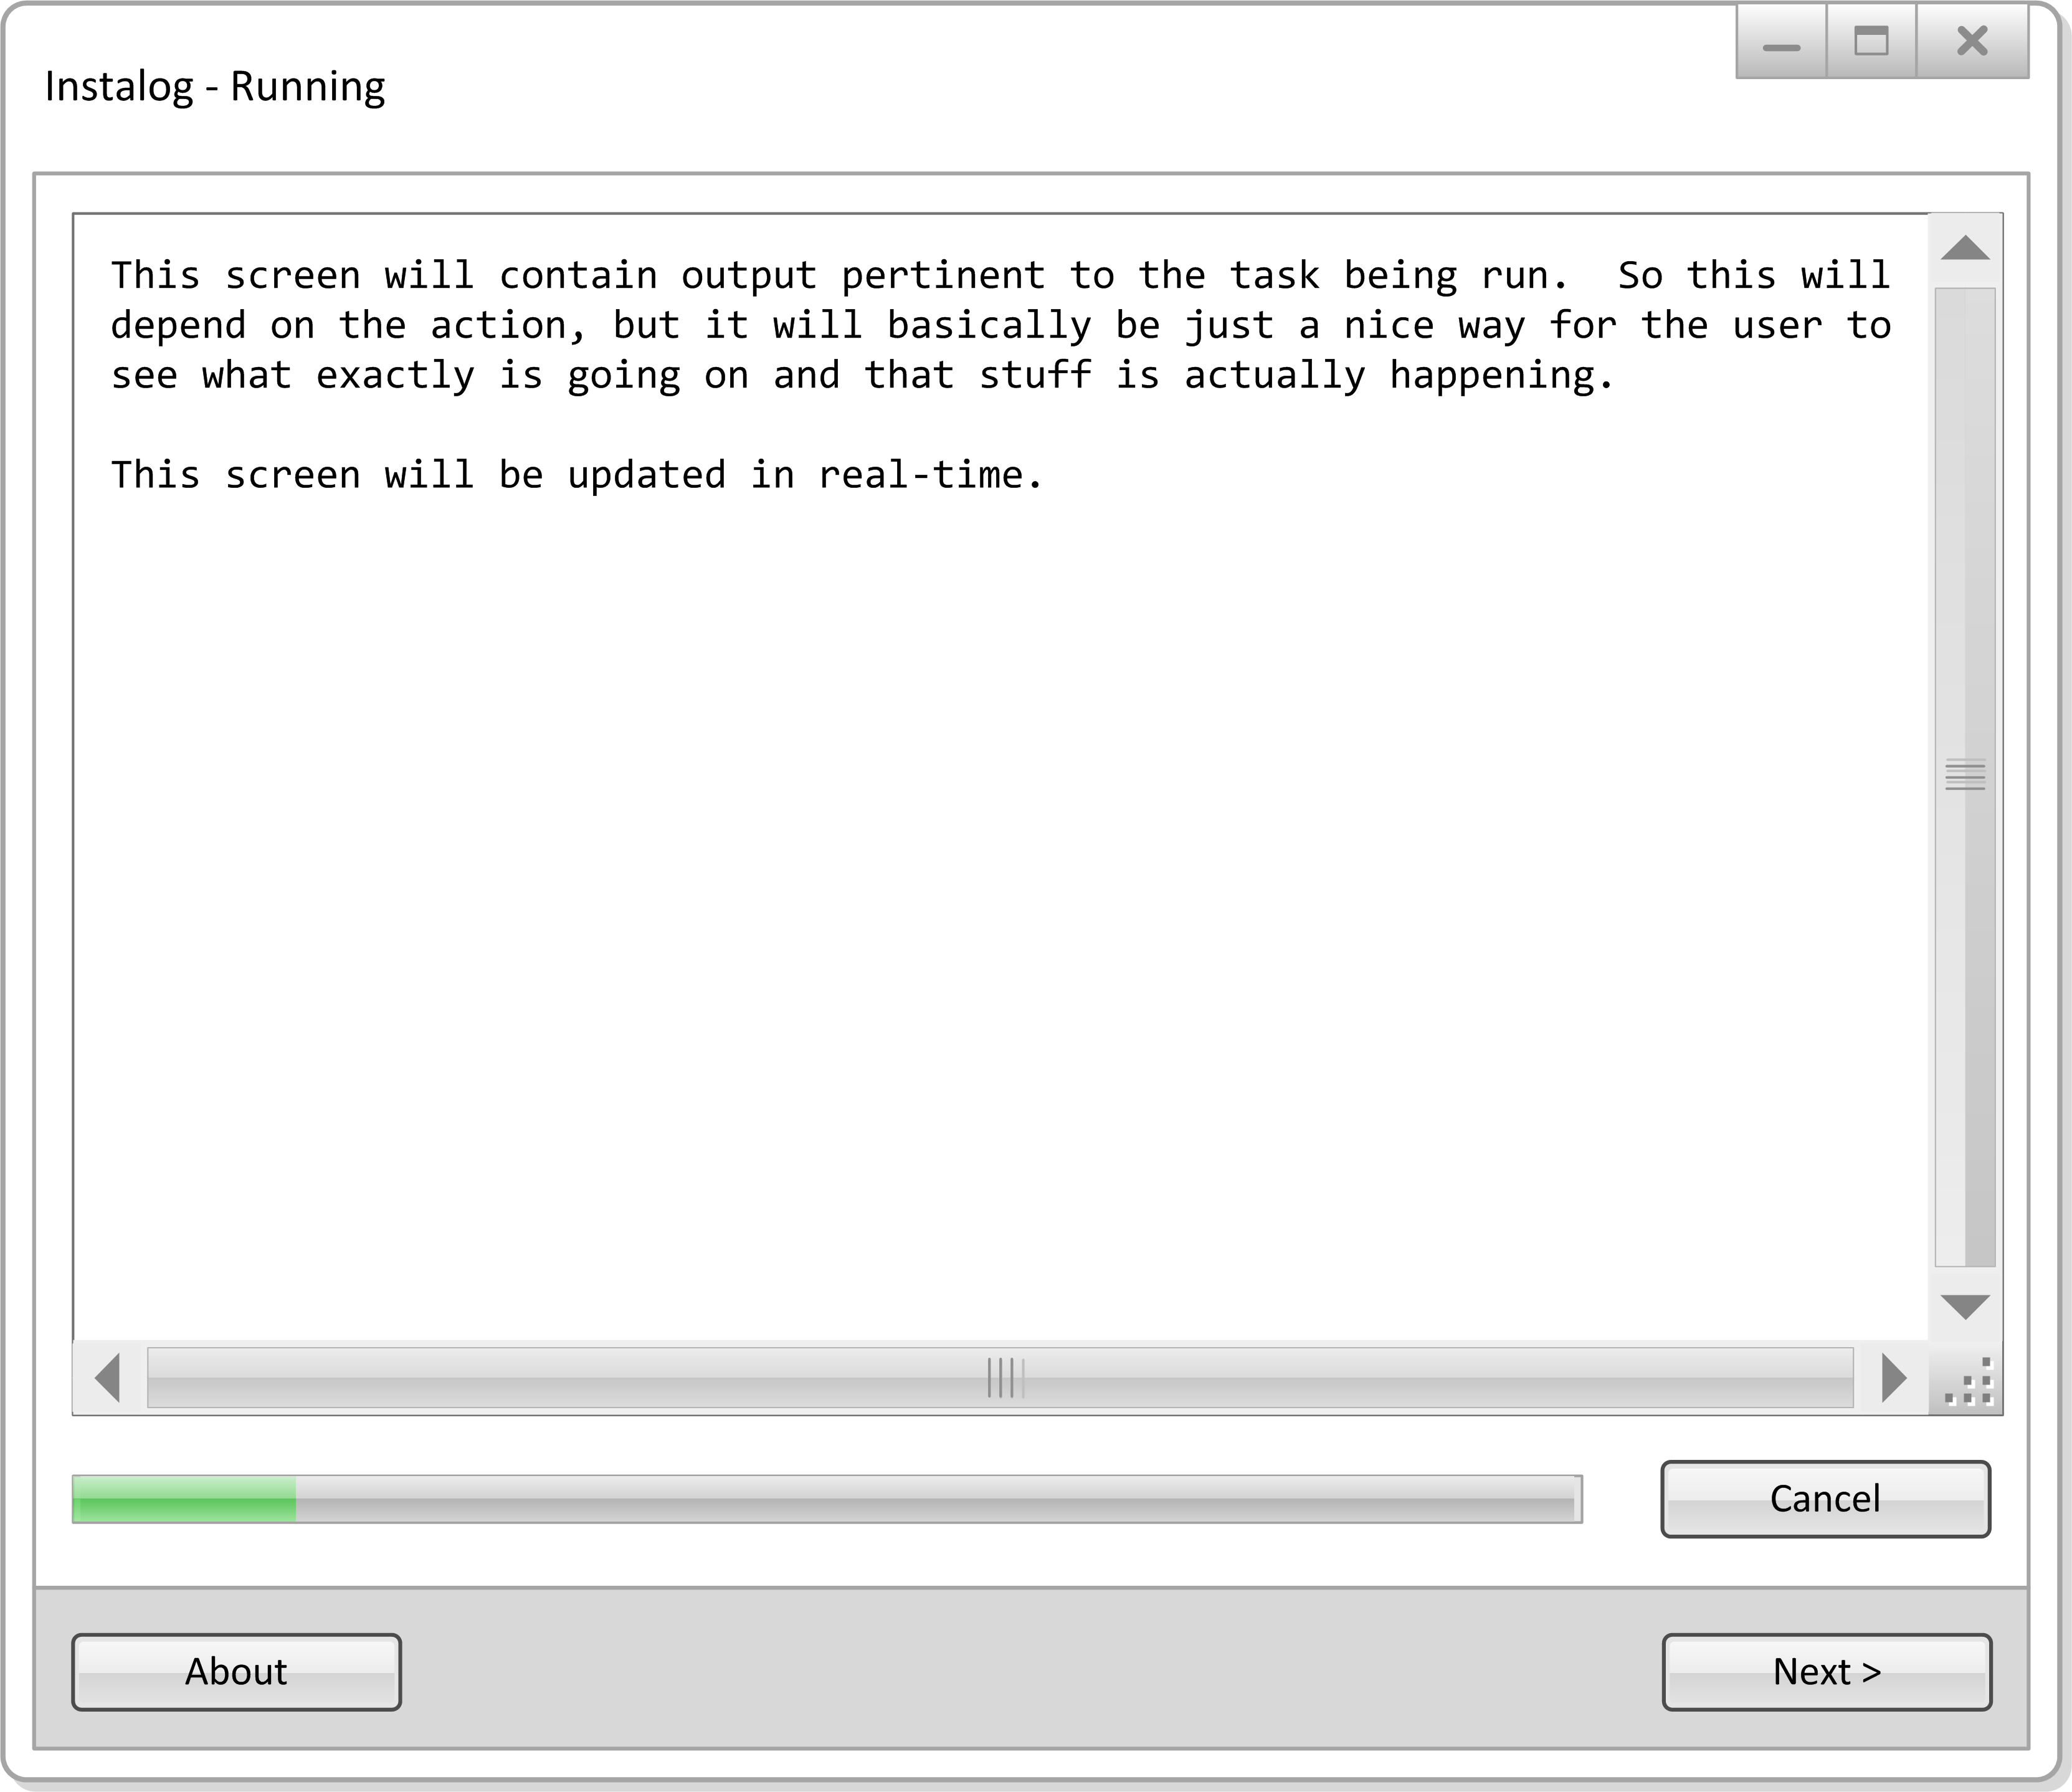
\includegraphics{figures/gui/Running.png}
  	\caption{GUI Running Screen}
  	\label{fig:gui_running}
\end{figure}

\begin{description}
\item[Textbox requirements] \hfill 
\begin{enumerate}
  \item The textbox shall be updated to display the (raw) log output of the
  currently running screen.  This textbox shall only be updated at a rate of 60
  Hz to avoid slowing down the GUI.
  \item The textbox must be scrollable.  It shall automatically scroll down to 
  follow the output by default.  If the user scrolls up for any reason, it shall
  no longer auto-scroll unless the user manually scrolls all the way down to the
  bottom of the output.
\end{enumerate}
\item[Progress bar requirements] \hfill 
\begin{enumerate}
  \item The progress bar shall contain the best estimate of the progress through
  the script.  This estimate can be something as simple as the completed script 
  actions divided by the total script actions.
\end{enumerate}
\item[Cancel button requirements] \hfill 
\begin{enumerate}
  \item The ``Cancel'' button must not be enabled if the script contains any 
  system-altering actions.  This can be determined by scanning the script in 
  advance.
  \item If the user presses the ``Cancel" button, the ``Next" button must  
  change to display ``Exit."  The text of the ``Cancel" button shall change to
  ``Re-run."  The behavior of both of these buttons should be self-explanatory.
  \item When the script completes, if the script was not a system-altering
  script, then the button should change to ``Re-run."  Otherwise, it shall
  remain displaying ``Cancel" and be disabled.
\end{enumerate}
\item[Window close button requirements] \hfill 
\begin{enumerate}
  \item The window close button must not be enabled if the script contains any 
  system-altering actions.  This can be determined by scanning the script in
  advance.
  \item If the user presses the window close button at any time that it is
  enabled, a Yes/No dialog should appear that reminds the user that the script
  output has not been saved yet.
\end{enumerate}
\item[Next button requirements] \hfill 
\begin{enumerate}
  \item The ``Next" button shall not be enabled until after the script 
  completes.
  \item When the user presses the ``Next" button, the tool shall proceed to the
  Run Completed Screen (section~\ref{sec:run_completed_screen}).
\end{enumerate}
\end{description}

\subsection{Run Completed Screen} \label{sec:run_completed_screen}
This screen enables a user to decide what to do with their script output (log
file).  This screen is presented in Figure~\ref{fig:gui_run_complete}.

\begin{figure}[h]
  	\centering
	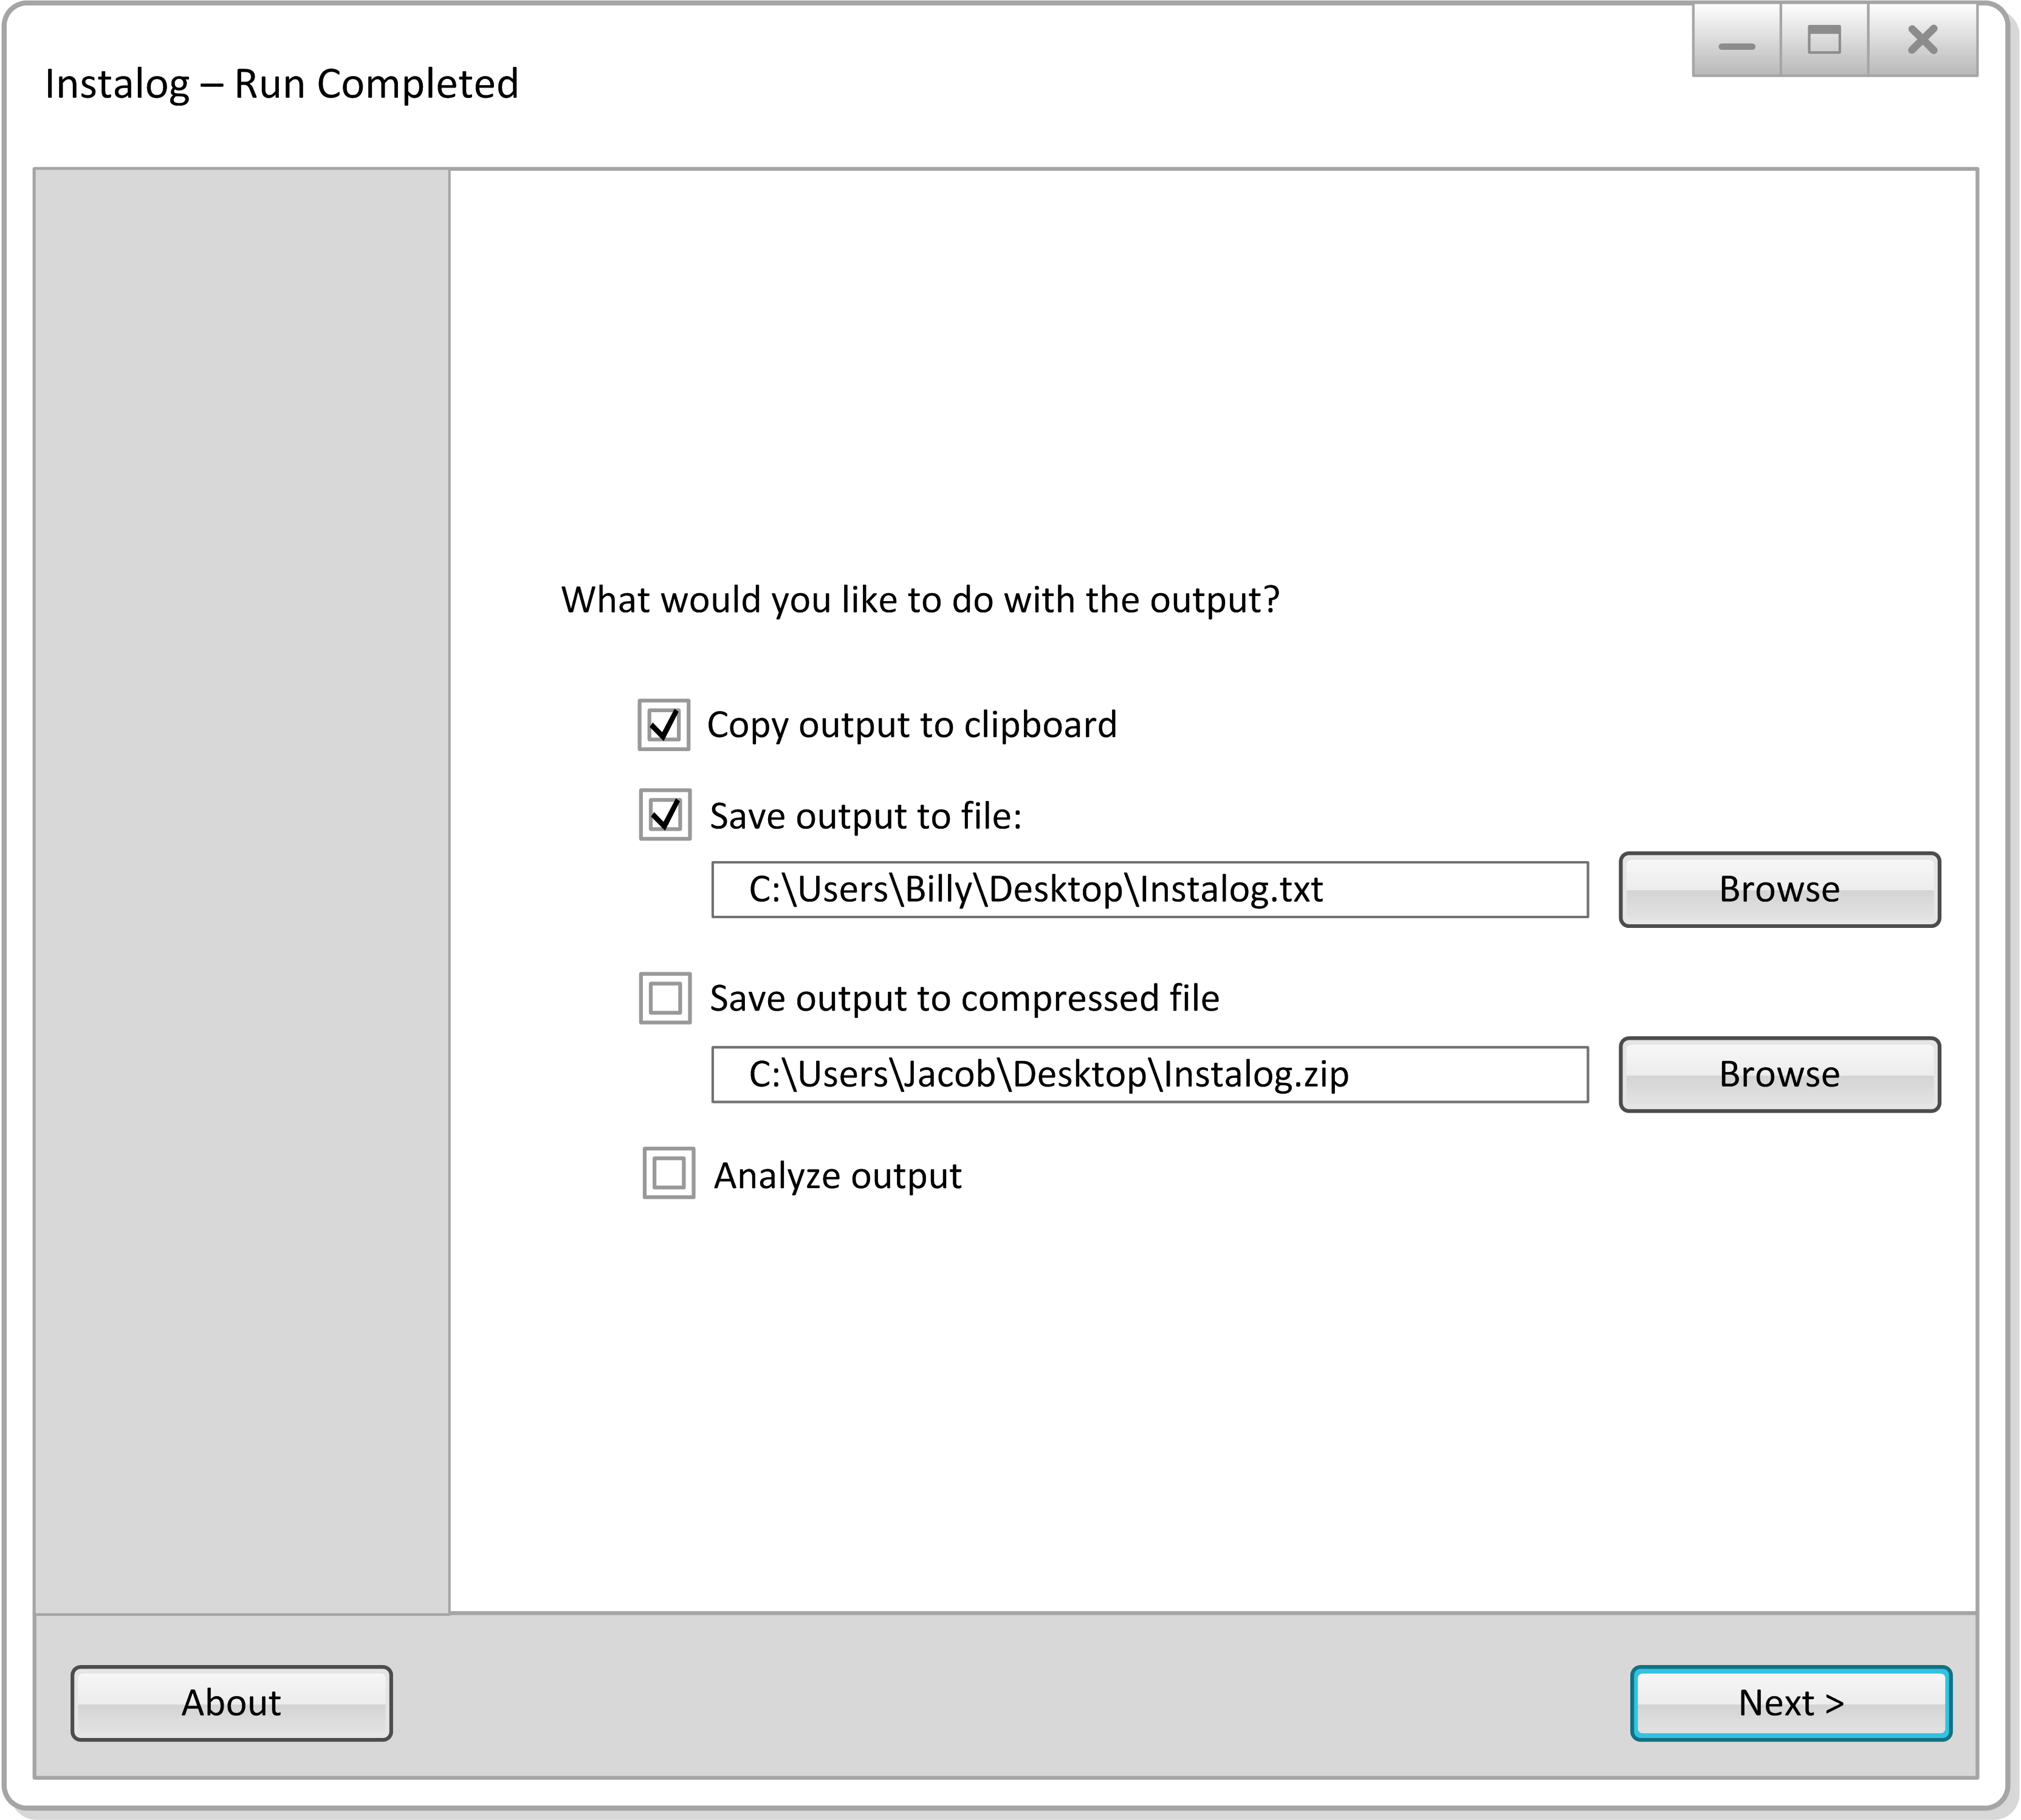
\includegraphics{figures/gui/Run_Completed.png}
  	\caption{GUI Run Complete Screen}
  	\label{fig:gui_run_complete}
\end{figure}

\begin{description}
\item[Option requirements] \hfill
\begin{enumerate}
  \item By default, nothing shall be selected
  \item Both of the file Save fields shall default to the user's desktop
  (\verb|%userprofile%\Desktop\|) with the filenames \verb|Log.txt| and
  \verb|Log.zip|.
\end{enumerate}
\item[Next button requirements] \hfill
\begin{enumerate}
  \item The button must be disabled until at least one option is selected. It
  must return to being disabled if nothing is selected.
  \item The button shall have the following behavior when it is clicked:
  \begin{enumerate}
    \item If the options selected did not include ``Analyze output," then the
    tool shall proceed to the Finished Screen
    (section~\ref{sec:finished_screen}).
    \item If the options selected include ``Analyze output" and other options,
    then the other options shall execute and then the tool should proceed to
    the Analysis Screen (section~\ref{sec:analysis_screen}).
    \item If the only option selected was ``Analyze output," then the tool
    shall proceed to the Analysis Screen (section~\ref{sec:analysis_screen})
    after displaying a warning that the output will be otherwise unsavable.
  \end{enumerate}
\end{enumerate}
\item[Window close button requirements] \hfill
\begin{enumerate}
  \item If the user presses the window close button at any time that it is
  enabled, a Yes/No dialog shall appear that reminds the user that the script
  output has not been saved yet.
\end{enumerate}
\end{description}


\subsection{Analysis Screen} \label{sec:analysis_screen}
The analysis screen enables users to construct a script based on the output
from a log.  For the requirements listed in this section, it does not
matter what workflow the user used to get to this screen.  This screen is
presented in figure~\ref{fig:gui_analyze}.

\begin{figure}[h]
  	\centering
	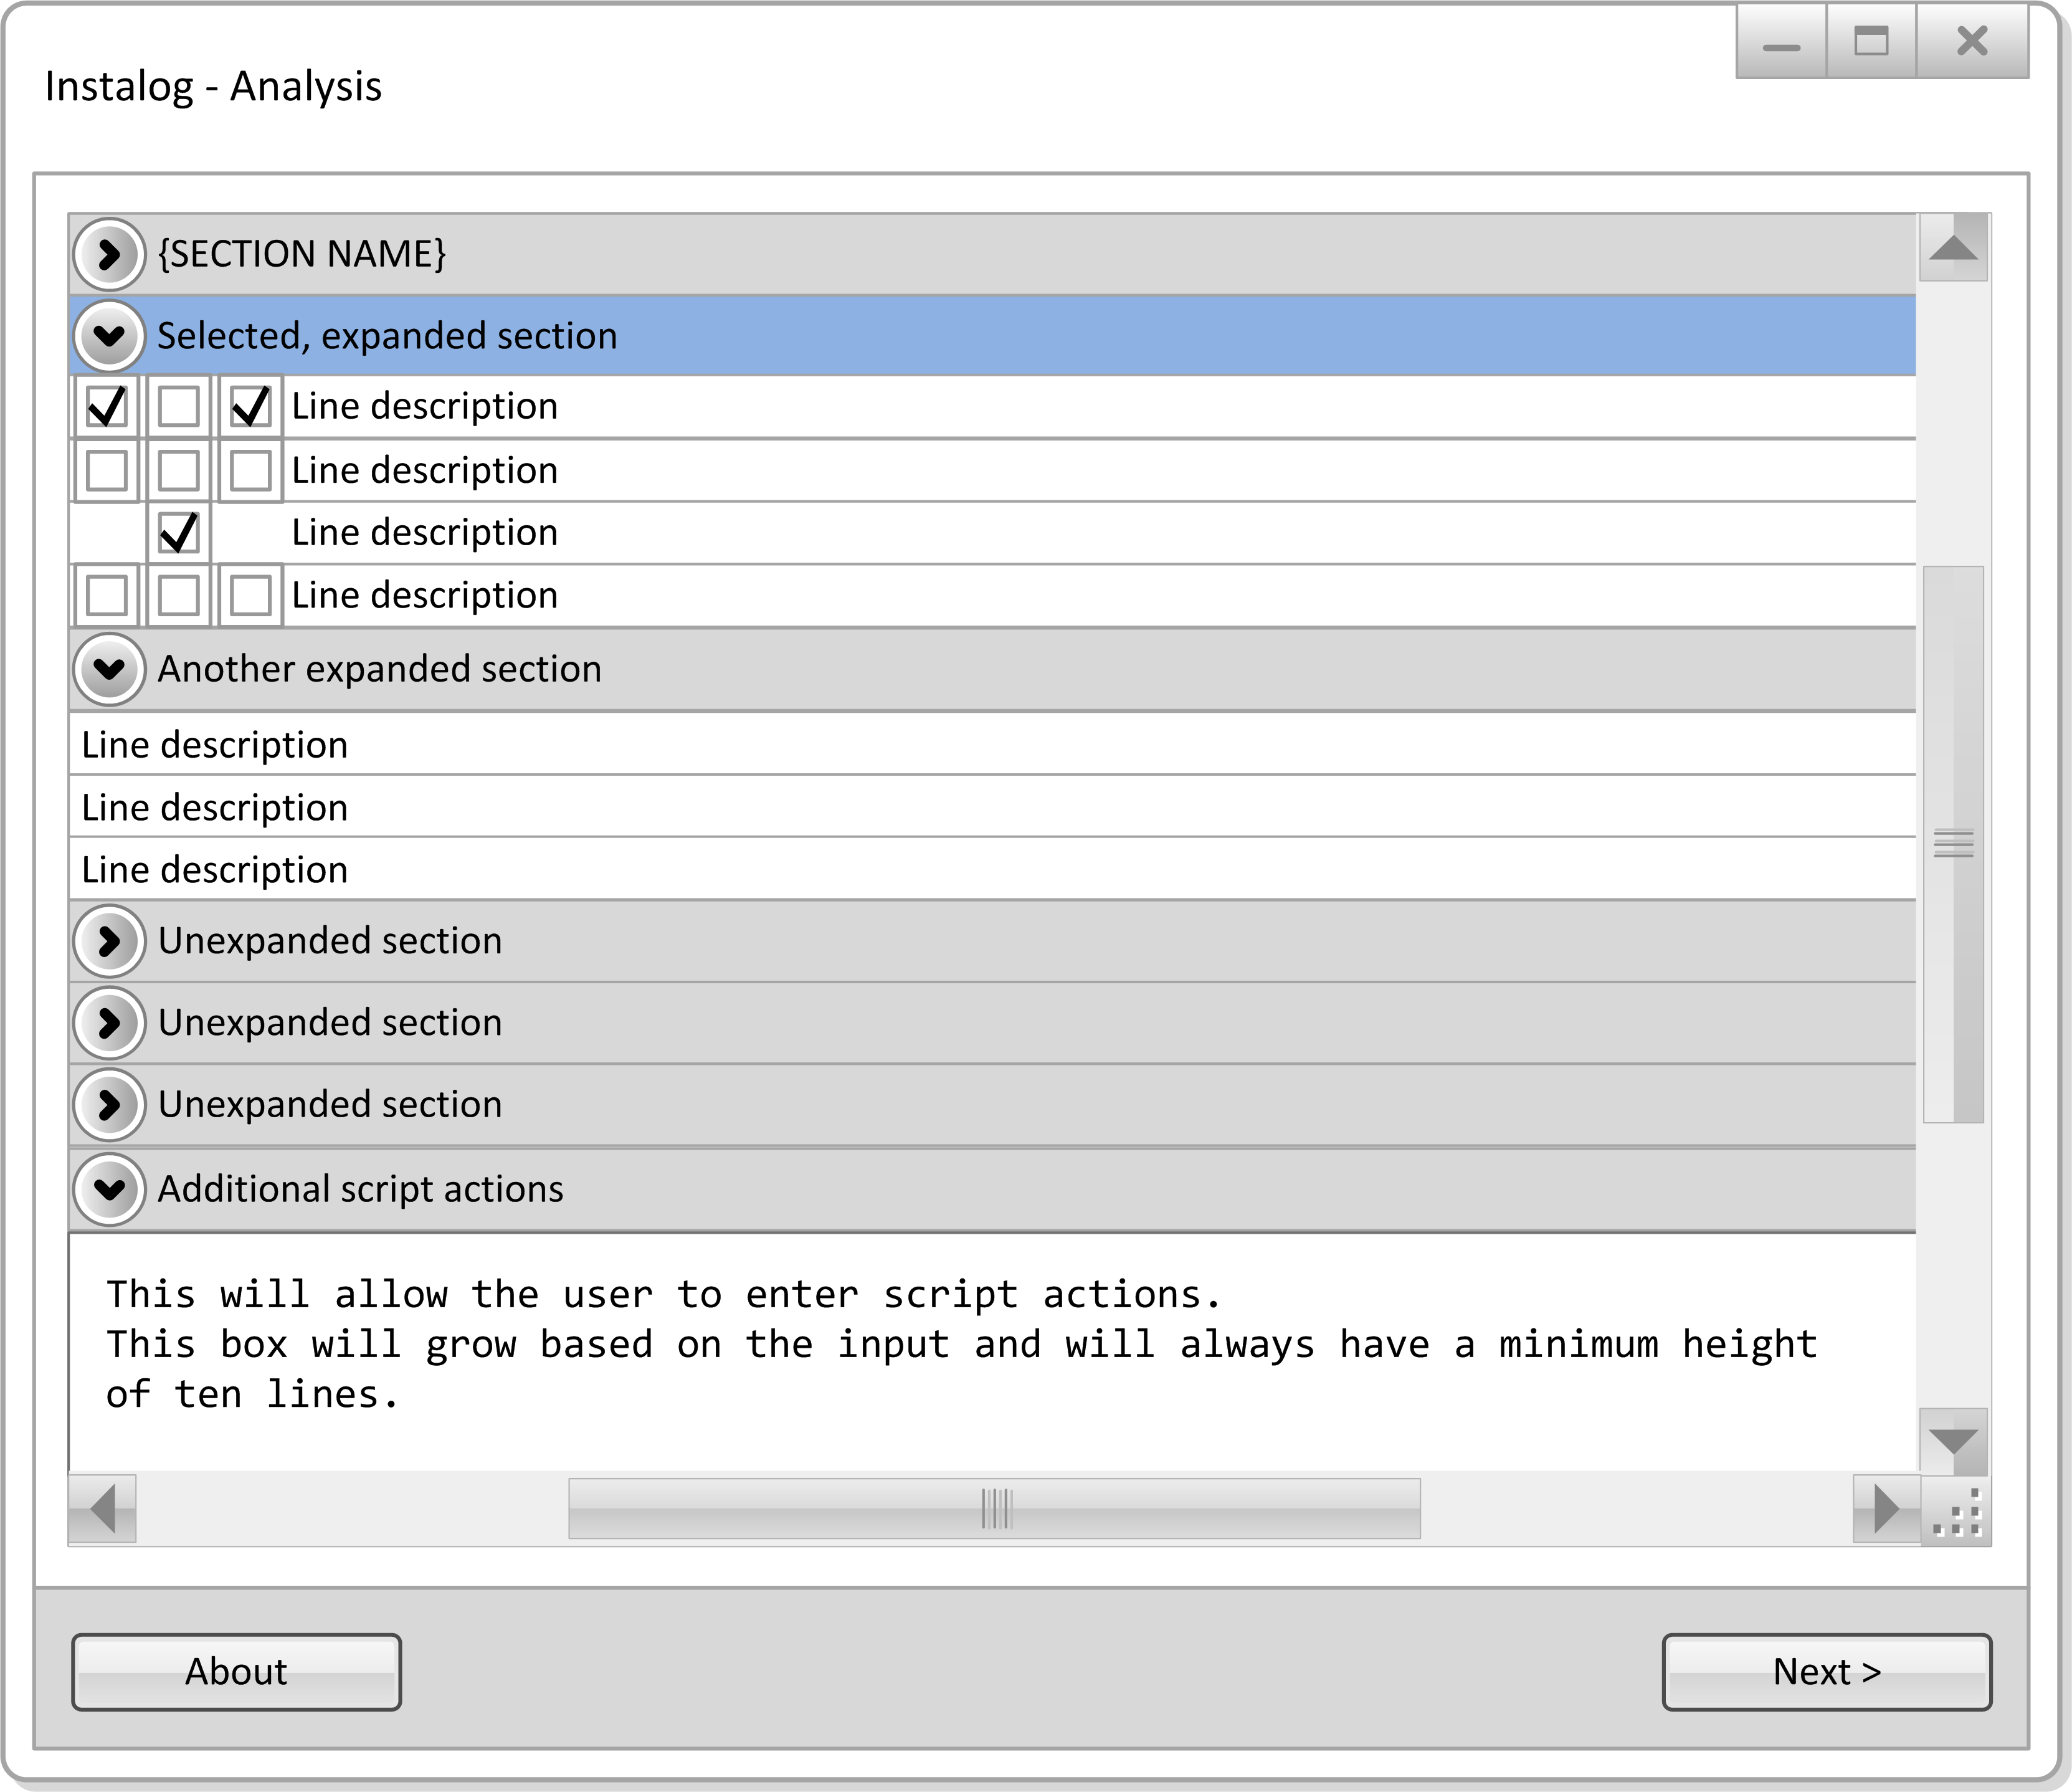
\includegraphics{figures/gui/Analysis.png}
  	\caption{GUI Analysis Screen}
  	\label{fig:gui_analyze}
\end{figure}

\begin{description}
\item[Section heading requirements] \hfill
\begin{enumerate}
  \item Each separate section in the log shall be parsed into one of the gray
  section.  Sections in the log are described in section~\ref{sec:log_output}.
  \item Sections can be collapsed or expanded by the user.  The user can either
  press the entire section heading or the Chevron arrow to perform this action.
  By default, all sections will be expanded.
  \item The Chevron arrow shall point to the right for collapsed sections and
  downward for expanded sections.
  \item No animation is necessary for the collapse action or expand action.
  \item Hovering over a section shall slightly change the background color.
  \item Each corresponding line shall be listed under the section.  Some
  sections might not have any lines.  In this case, a single line shall appear
  with the following text in italics: ``No lines available for this section."
\end{enumerate}
\item[Line requirements] \hfill
\begin{enumerate}
  \item Each separate line of the log will be logged into a line underneath the
  corresponding section.
  \item Hovering over a line shall slightly change the background color.
\end{enumerate}
\item[Checkbox requirements] \hfill
\begin{enumerate}
  \item Depending on the line, there may be zero, one, or many actions available
  for the given line.  There shall be a checkbox to the left of the line for
  each action.  Checking a box indicates that the action shall be taken.
  \item A user shall be able to hover their mouse over any checkbox to
  determine what action the checkbox enables.
  \item In a given section, actions shall be grouped by actions.  Therefore,
  each column will only have one type of action in it.  If an action does not
  apply to a line, there shall simply be an empty slot where the checkbox would
  be.
  \item All checkboxes shall default to unchecked.
\end{enumerate}
\item[Aditional script actions requirements] \hfill
\begin{enumerate}
  \item The last section in the log must always be titled ``Additional script
  actions'' and will contain a textbox that will allow the user to specify
  additional script actions to take
  \item The textbox shall always have a minimum height of ten lines and will
  grow to always be one line longer than its contents
  \item The textbox shall not have its own scrollbars.  Rather, the scrollbars
  for the rest of the control are be sufficient
  \item The textbox must support basic operations including but not limited
  to Copy, Paste, and Undo/Redo.
  \item The textbox shall not implement word-wrap.
\end{enumerate}
\item[Next button requirements] \hfill
\begin{enumerate}
  \item The Next button shall display a Yes/No dialog warning the user that
  scripts are final and there is no going back.
\end{enumerate}
\end{description}

\subsection{Analysis Completed Screen}
This screen enables a user to decide what to do with the finished script.  This
screen is presented in Figure~\ref{fig:gui_analysis_completed}.

\begin{figure}[h]
  	\centering
	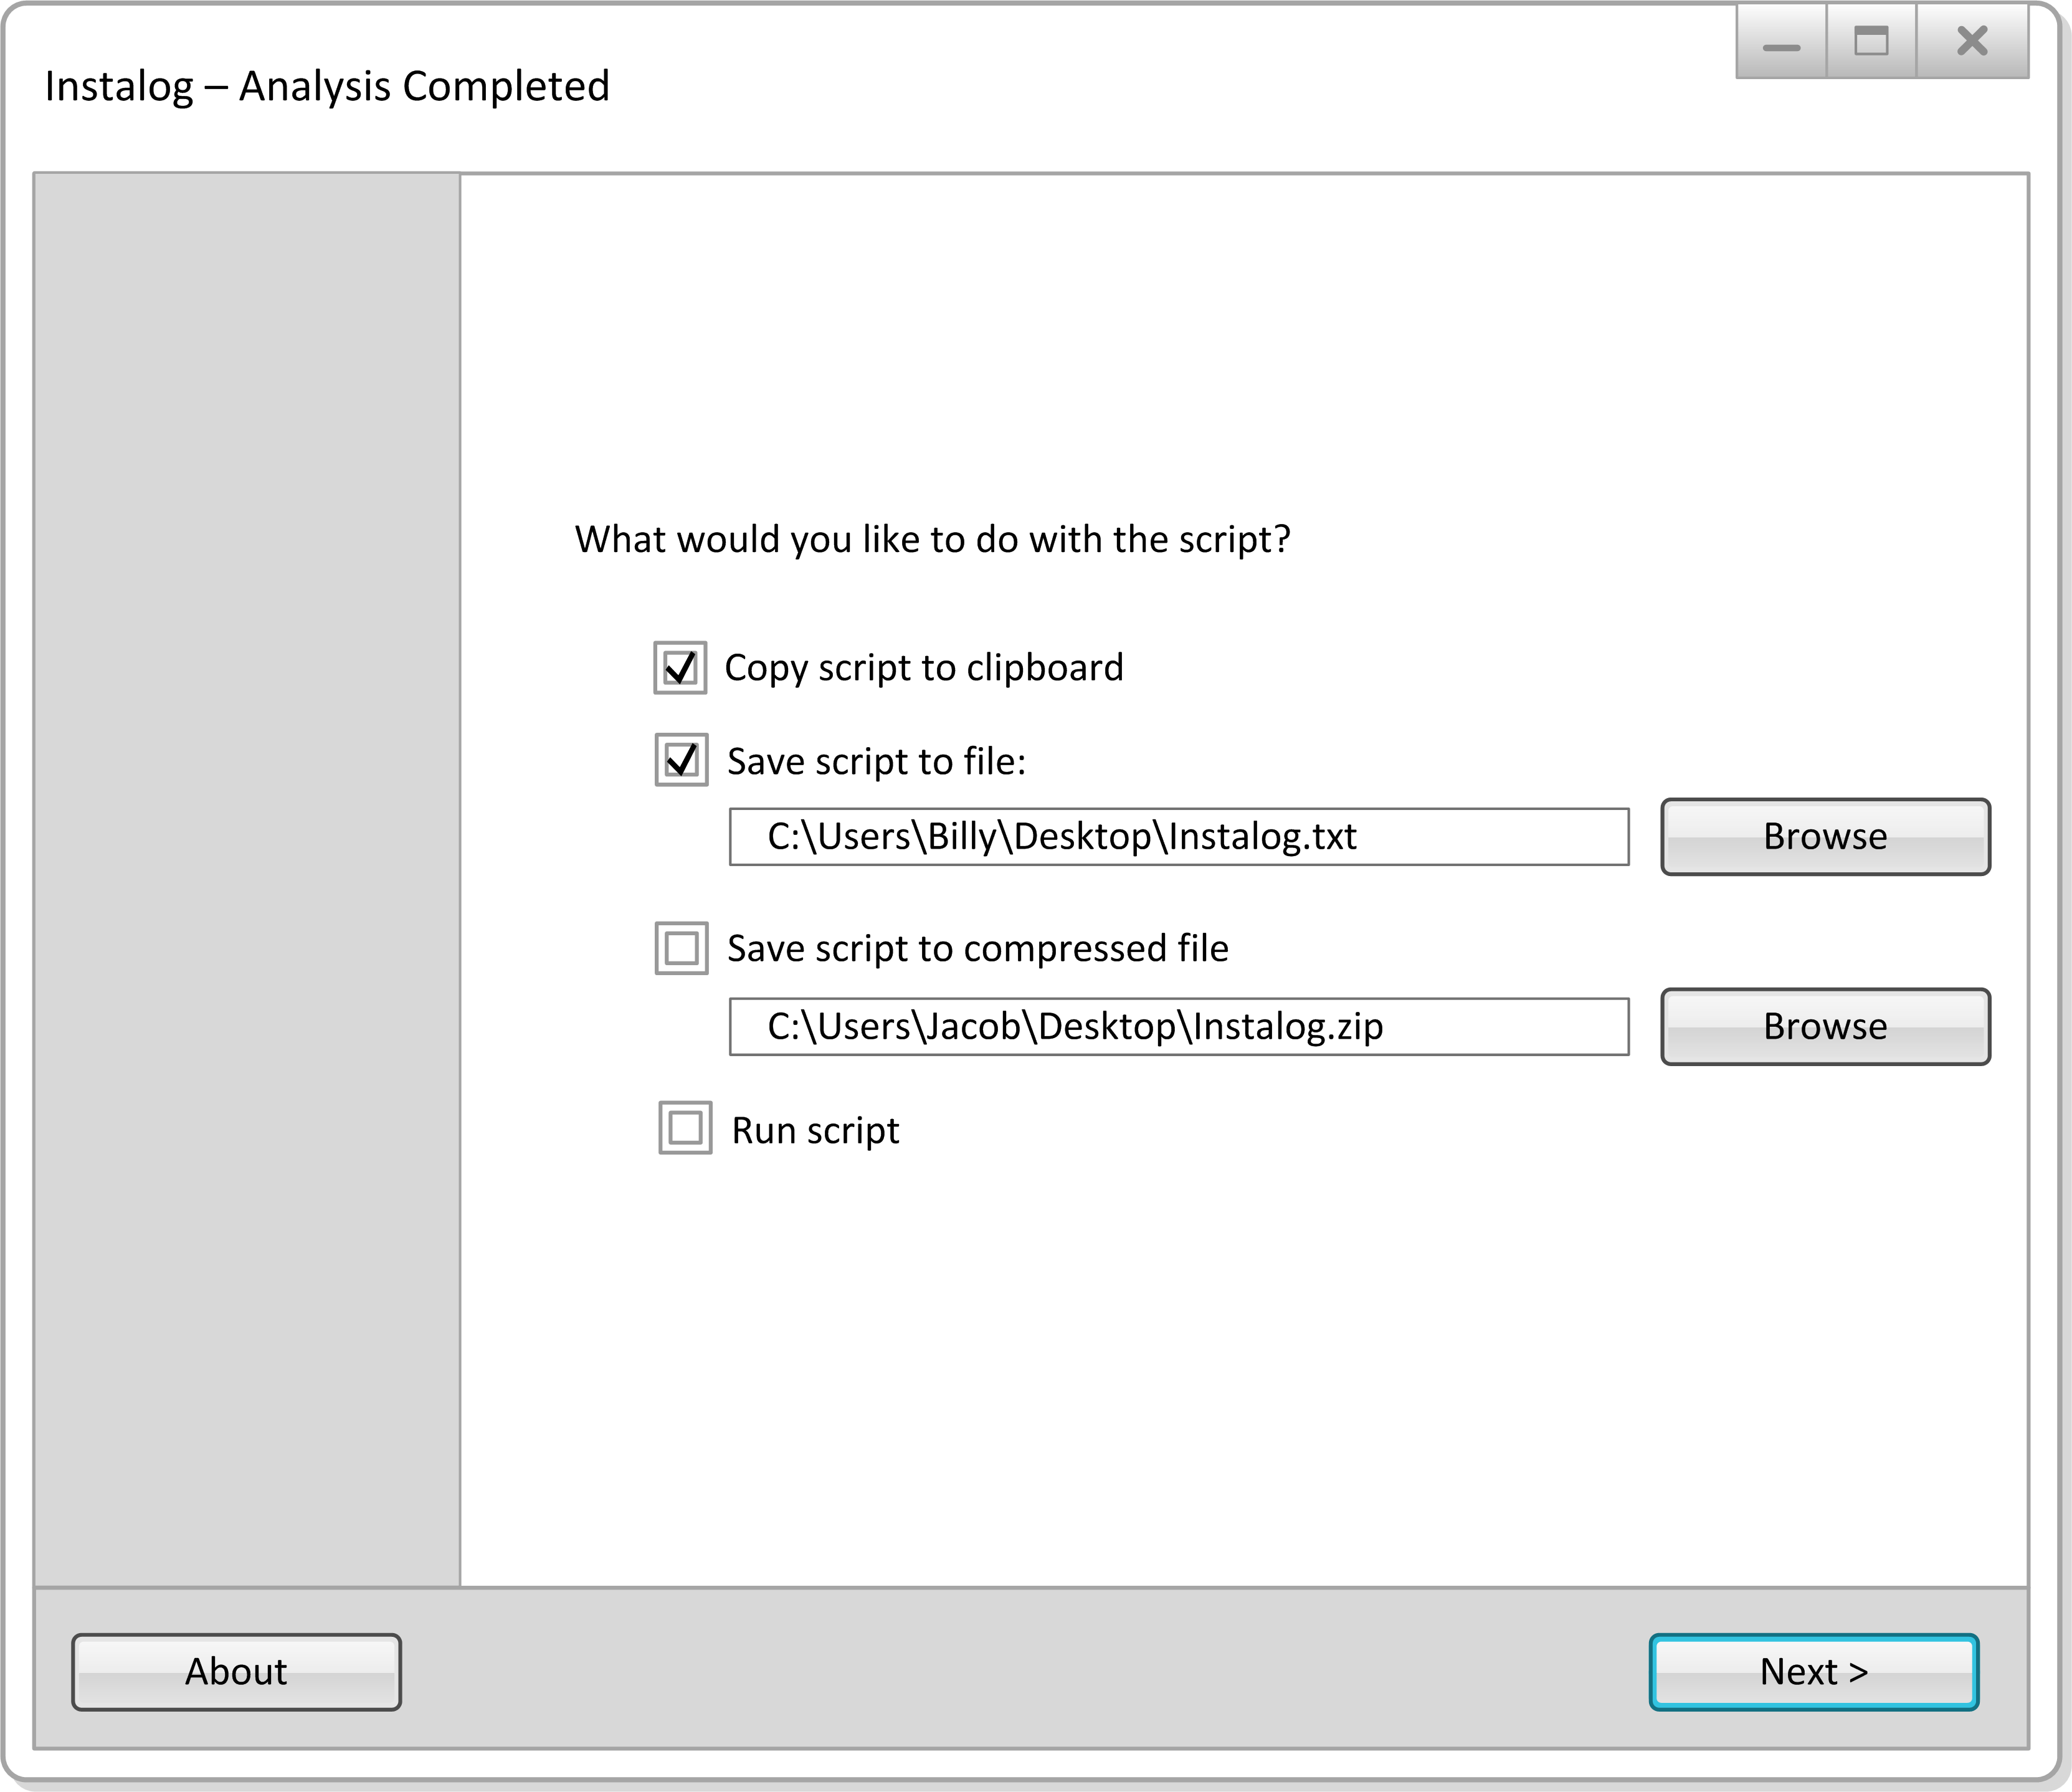
\includegraphics{figures/gui/Analysis_Completed.png}
  	\caption{GUI Analysis Completed Screen}
  	\label{fig:gui_analysis_completed}
\end{figure}

\begin{description}
\item[Option requirements] \hfill
\begin{enumerate}
  \item By default, nothing shall be selected
  \item Both of the file Save fields shall default to the user's desktop
  (\verb|%userprofile%\Desktop\|) with the filenames \verb|Script.txt| and
  \verb|Script.zip|.
\end{enumerate}
\item[Next button requirements] \hfill
\begin{enumerate}
  \item The button must be disabled until at least one option is selected. It
  must return to being disabled if nothing is selected.
  \item The button shall have the following behavior when it is clicked:
  \begin{enumerate}
    \item If the options selected did not include ``Run script," then the tool
    shall proceed to the Finished Screen (section~\ref{sec:finished_screen}).
    \item If the options selected include ``Run script" and other options, then
    the other options shall execute and then the tool shall proceed to the
    Running Screen (section~\ref{sec:running_screen}).
    \item If the only option selected was ``Run script," then the tool shall
    proceed to the Running Screen (section~\ref{sec:running_screen}).
  \end{enumerate}
\end{enumerate}
\item[Window close button requirements] \hfill
\begin{enumerate}
  \item If the user presses the window close button at any time that it is
  enabled, a Yes/No dialog must appear that reminds the user that the script
  has not been saved yet.
\end{enumerate}
\end{description}

\subsection{Finished Screen} \label{sec:finished_screen}
The finished screen provides the user with some confirmation that the actions
instructed of the tool were actually executed.  This is to prevent users from
becoming disoriented and thinking that the tool had crashed or something else
bad had happened.  This screen is presented in Figure~\ref{fig:gui_finished}.

\begin{figure}[h]
  	\centering
	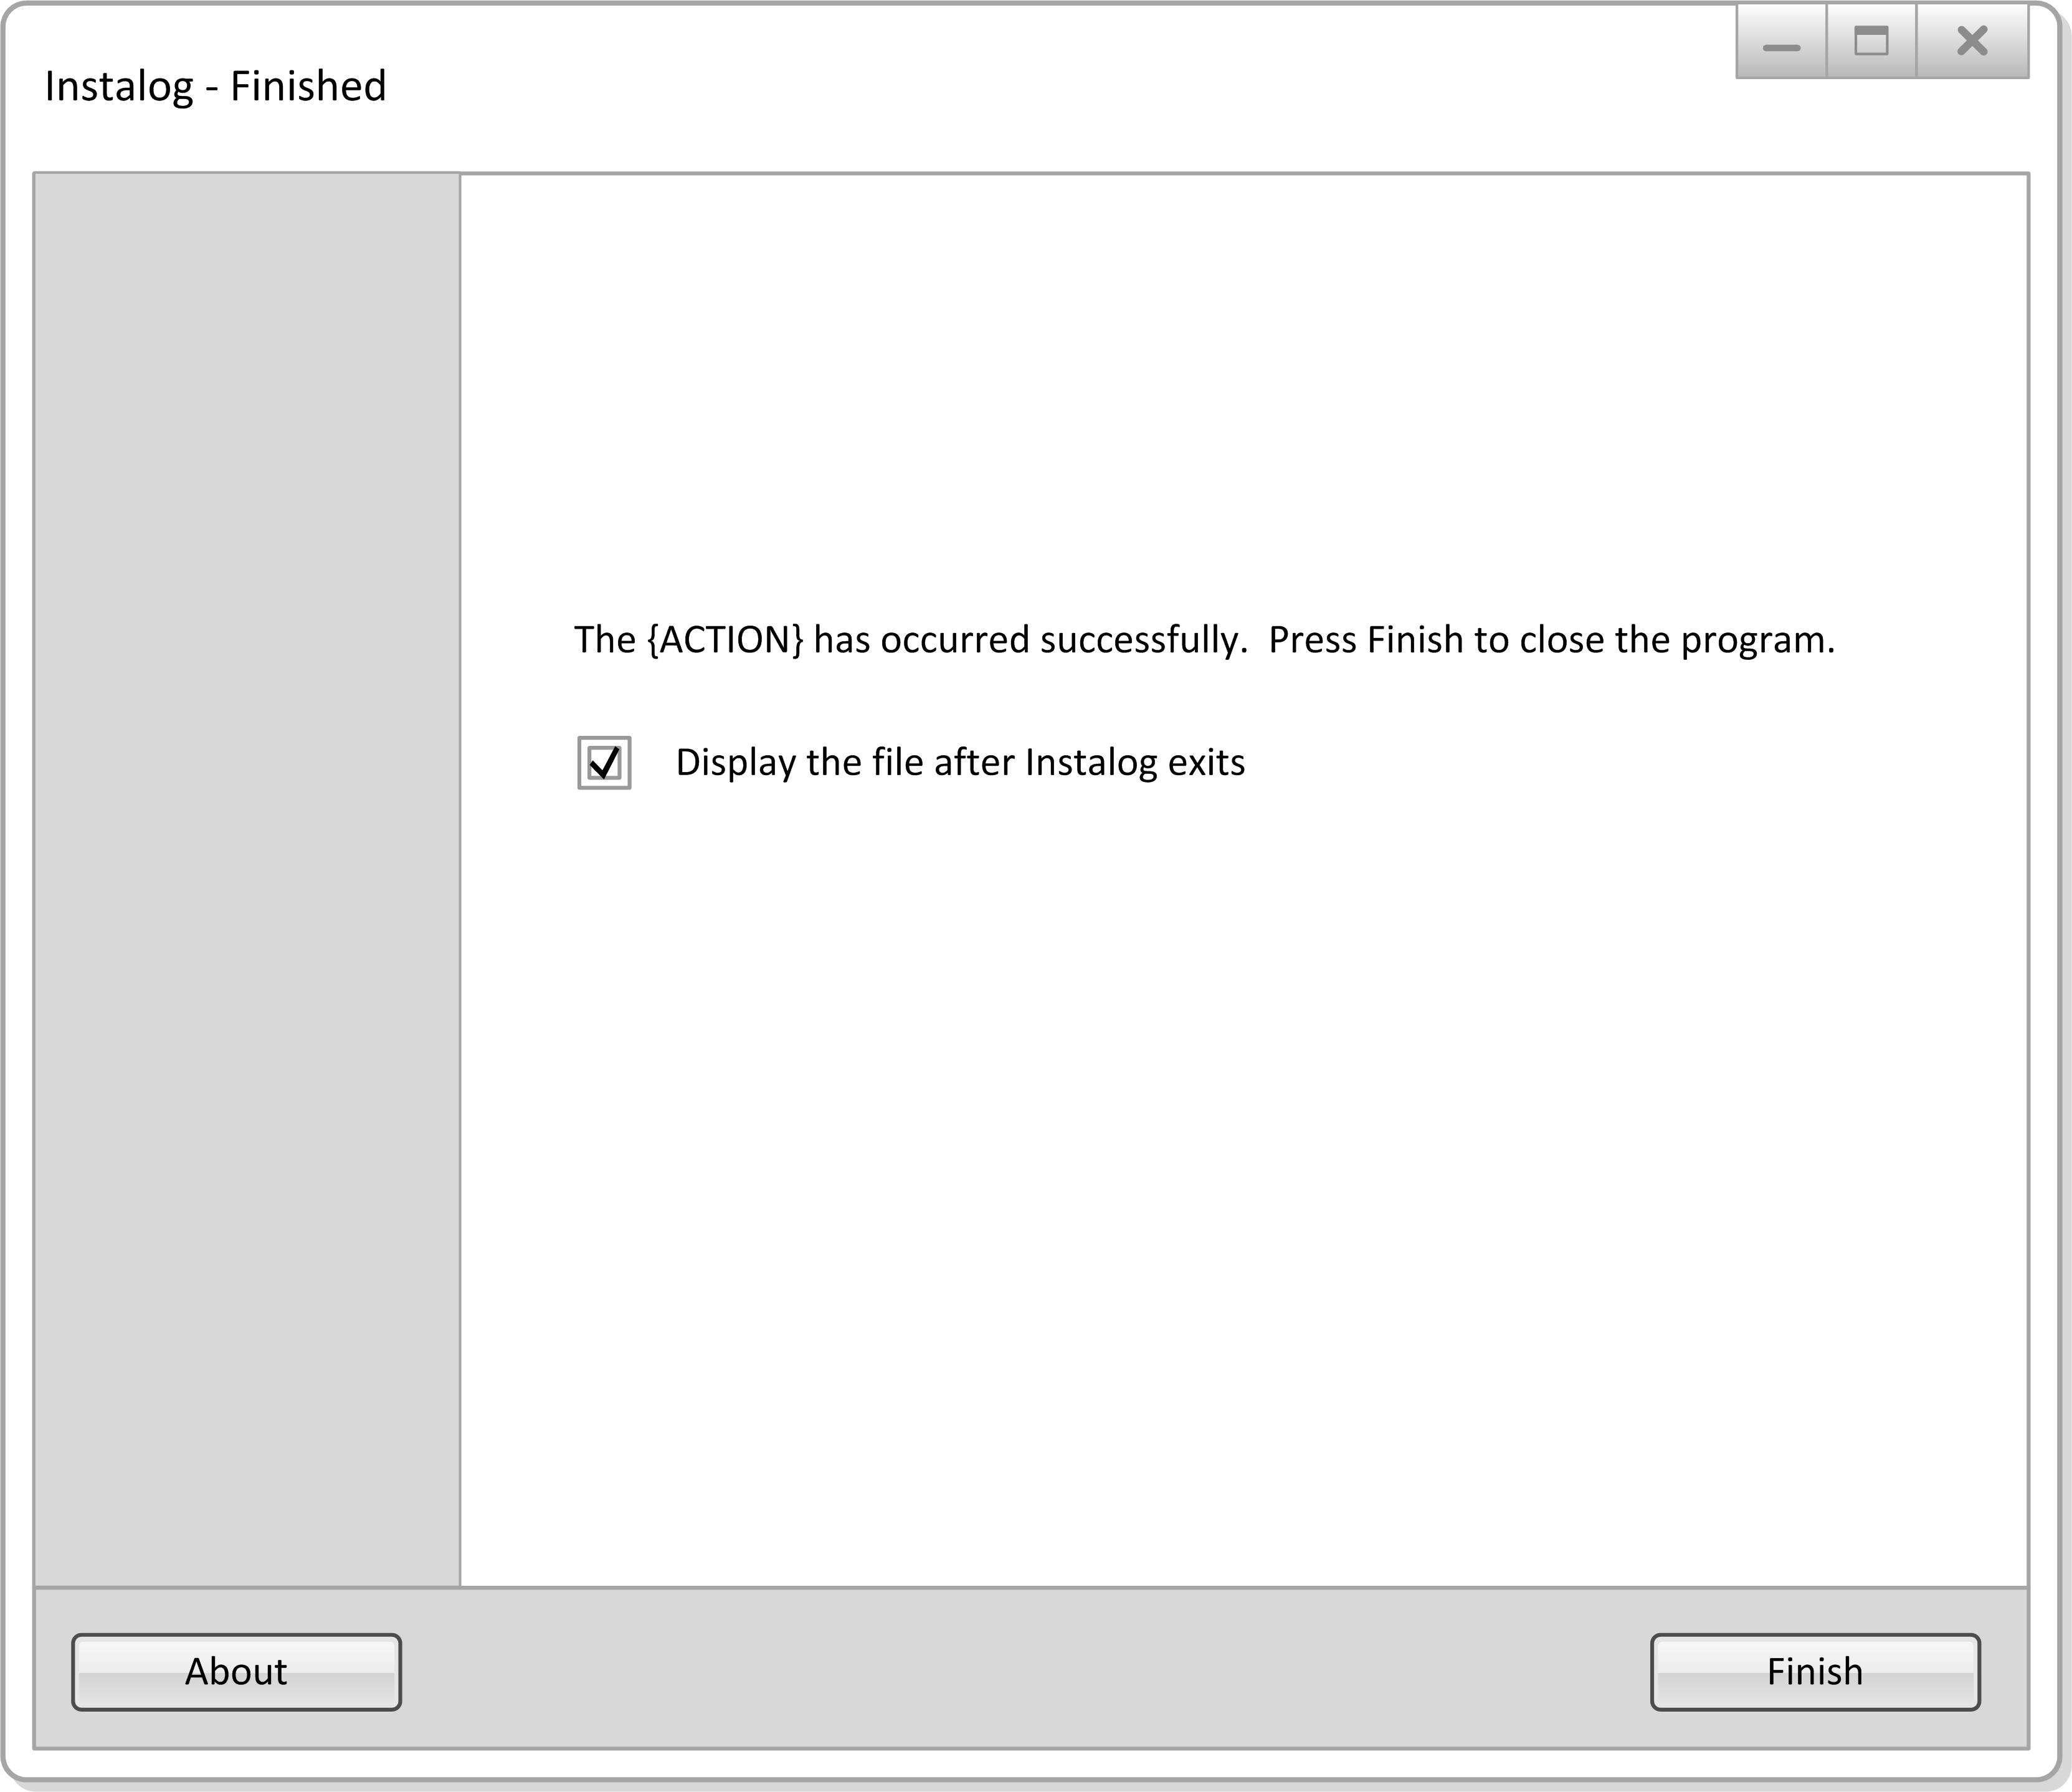
\includegraphics{figures/gui/Finished.png}
  	\caption{GUI Finished Screen}
  	\label{fig:gui_finished}
\end{figure}

\begin{description}
\item[Text requirements] \hfill
\begin{enumerate}
  \item The text shall display some information about what happened.  The text
  should cover all possible combinations of copying material to the clipboard,
  saving one file, or saving two files.
\end{enumerate}
\item[Display file checkbox requirements] \hfill
\begin{enumerate}
  \item If a plaintext file was saved, then a checkbox shall be displayed that
  allows the user to specify if they want to view the file when the program
  exits.
  \item The default state of this checkbox shall be unchecked.
  \item Upon exiting, if this is checked, notepad shall be launched and display
  this file.
\end{enumerate}
\end{description}

\subsection{Flowchart}
Since there are several different branch points in the tool, the flow through
the tool is difficult to describe by simply using text.  The flow described in
the preceding sections is described in Figure~\ref{fig:gui_flowchart} in
flowchart form.

\begin{figure}[h!]
  	\centering
	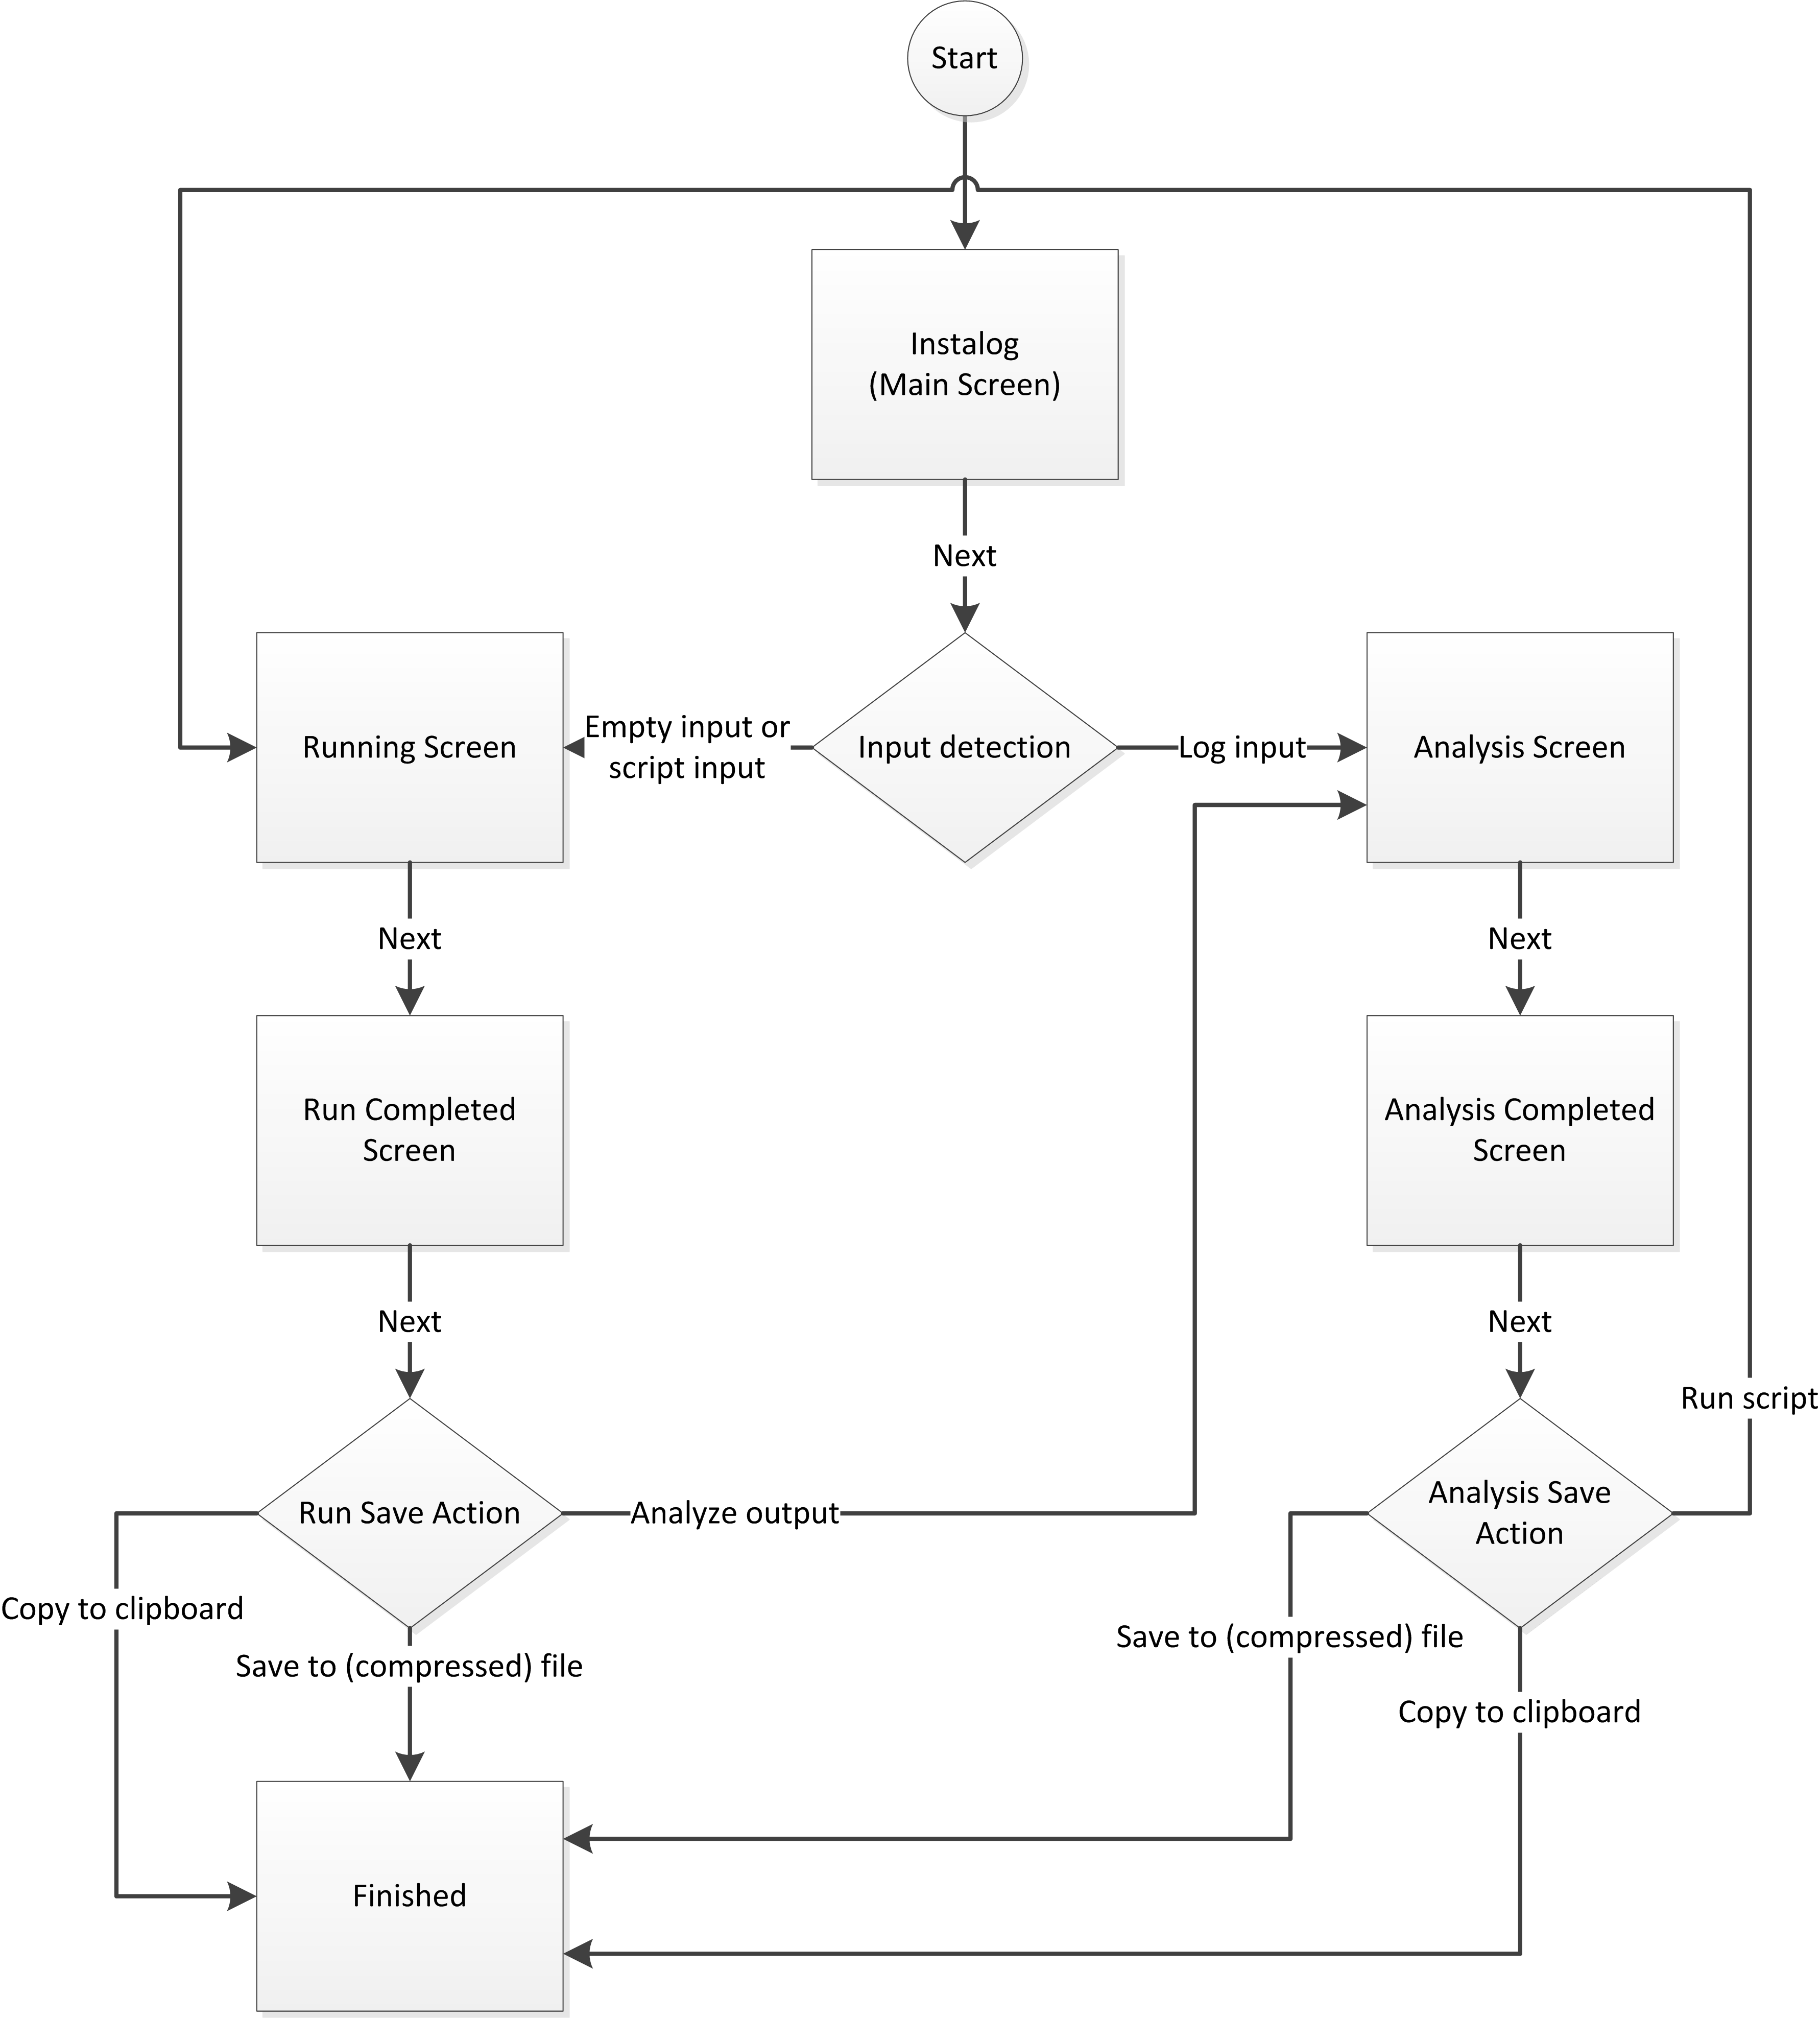
\includegraphics{figures/gui/GUI_Flowchart.png}
  	\caption{GUI Flowchart}
  	\label{fig:gui_flowchart}
\end{figure}